\documentclass[12pt]{article}
\usepackage{amsmath,geometry,times,bm,float}
\geometry{margin=1.00in}
\floatplacement{figure}{H}

\title{Math 297 Project I}
\author{Jiaqi Liu}\date{12 February 2022}
\usepackage{Sweave}
\begin{document}\maketitle\thispagestyle{empty}
\Sconcordance{concordance:Project1.tex:Project1.Rnw:%
1 7 1 1 0 2 1 1 2 1 0 9 1 3 0 1 2 4 1 1 15 17 0 2 2 1 0 1 1 3 0 1 2 4 1 %
1 2 1 0 1 3 5 0 1 2 1 7 45 1 1 2 1 0 2 1 3 0 1 2 5 1 1 2 1 0 3 1 1 23 %
22 0 2 1 1 2 4 0 1 2 10 1 1 2 1 0 5 1 1 21 20 0 2 1 1 2 4 0 1 2 9 1 1 2 %
1 0 4 1 1 21 20 0 2 1 1 2 4 0 1 2 8 1}

First, let us load useful packages and data. Our data has one predictor and one response variables.
\begin{Schunk}
\begin{Sinput}
> library(tidyverse)
> require(lspline)
> require(splines)
> require(MASS)
> tmp <- read_csv("//Users/liujiaqi/Library/Mobile Documents/com~apple~CloudDocs/Math 297/tmp-20160413.csv")
> tmp = as.data.frame(tmp)
> names(tmp) = c("xx","yy")
> dat = tmp
> attach(dat)
> n = length(xx)
\end{Sinput}
\end{Schunk}


\section{Regressogram}
In this section, we are going to fit the data using the regressogram and identify the optimal number of bins. To begin with, we write a function which computes the residual sum of squares under regressogram models with different number of bins.

\begin{Schunk}
\begin{Sinput}
> regressores <- function(x, y, nbins){
+   xy <- data.frame(x=x, y=y)
+   xy <- xy[order(xy$x),]
+   z <- cut(xy$x,breaks=seq(min(xy$x),max(xy$x),length=round(nbins)+1),
+            labels=1:round(nbins),include.lowest=TRUE)
+   xyz <- data.frame(xy,z=z)
+   MEANS <- c(by(xyz$y,xyz$z,FUN=mean))
+   new = split(xyz, xyz$z)
+   res = 0
+   for (i in 1:round(nbins)){
+     res = res + sum((new[[i]][["y"]]-MEANS[i])^2)
+   }
+   return(res)
+ }
\end{Sinput}
\end{Schunk}
Next we estimate the variance $\sigma^2=var(Y|X)$. Consider a regressogram model with a very large number of bins $k_1=n/\log n$. The variance under this model can be estimated by the following procedure.
\begin{Schunk}
\begin{Sinput}
> k1 = round(n/log(n))
> sigmahat = regressores(xx, yy, k1)/(n-k1)
\end{Sinput}
\end{Schunk}
Therefore,
\[
\widehat\sigma^2 = 0.986199246346988.
\]
Finally, we calculate the estimated risks of the regressogram models with different number of bins
\begin{Schunk}
\begin{Sinput}
> regressrisk = rep(0, times = k1)
> for (i in 1:k1){
+   regressrisk[i] = regressores(xx, yy, i)/n +2*sigmahat*i/n
+ }
\end{Sinput}
\end{Schunk}
Ploting estimated risk as a function of the number of bins, 
The optimal number of bins is $42$.
\begin{figure}
\begin{center}
\caption{Estimated risks of the regressogram models with different number of bins}
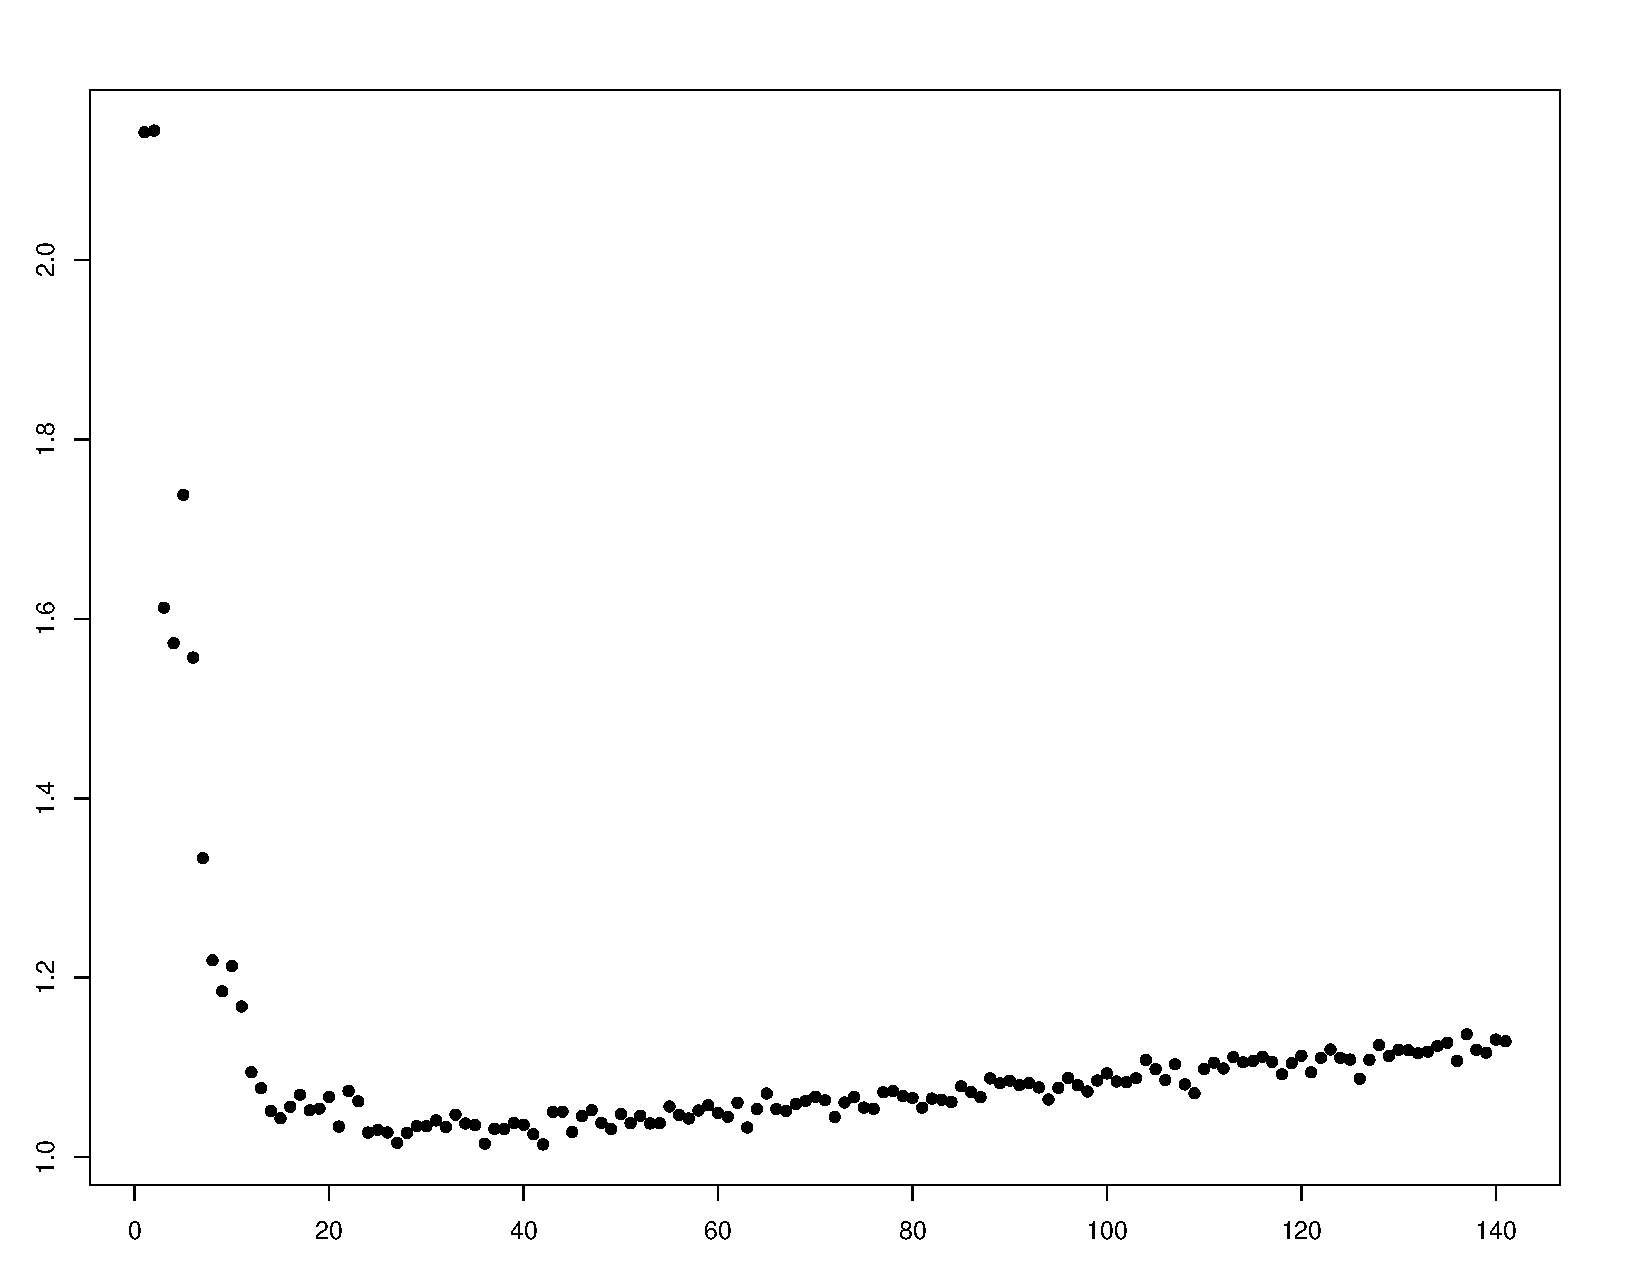
\includegraphics[scale=0.50]{figure1}
\end{center}
\end{figure}


\section{Paper summary}
Efron studied the relationship between two theories concerning the prediction error. The first theory is the penalty method which based on the covariance between data points and the corresponding predictions. The second theory is the cross validation which based on the nonparametric bootstrap techniques. As a byproduct, Efron also derived a general covariance penalty formula for a wide class of error measures, which can be used to determine the optimal degrees of freedom in variant models. Finally, a small simulation case is studied to illustrate covariance penalty and cross-validation relationships. 

Consider a homoskedastic model
\[
\bm{y}\sim (\bm{\mu},\sigma^2 I),
\]
which represents that each component $y_i$ has mean $\mu_i$ and variance $\sigma^2$, and all components are uncorrelated. Our goal is to estimate $\mu$ using the estimation rule
\begin{equation}
\widehat{\bm{\mu}}=m(\bm{y}).
\end{equation}
For a concave function $q(\dot)$ which measures the error, define $Err=(Err_i)_{i=1}^{n}$ to be the expectation of the assessed error for outcome $y$ given prediction $\widehat{mu}$
\[
Err_i=E_{o}(Q(y_i^o,\widehat{\mu}_i))=E_{o}(q(\widehat{mu}_i)+\dot{q}(\widehat{\mu}(y_i^o)-\widehat{\mu})-q(y_i^o))
\]
where $\widehat{\mu}_i$ is fixed in the expectation and $\bm{y}^o$ is an independent copy of $\bm{y}$. According to the optimism theorem, an unbiased estimator of $Err_i$ is the summation of the estimation error $err_i$ and the covariance penalty
\[
Err_i=err_i+2cov(\widehat{\lambda}_i,y_i)=Q(y_i,\widehat{\mu}_i)+2cov(-\dot{q}(\widehat{\mu}_i)/2,y_i).
\]
The convariance penalty can be calculted by the parametric bootstrap. Assume $\bm{y}\sim N(\widehat{\bm{\mu}},\widehat{\sigma}^2I)$ where $\widehat{\bm{\mu}}$ can be estimated as in (1) and $\widehat{\sigma}^2$ can be estimated from the residuals of some model with a very large degree of freedom. For $i=1,...,n$, generate a large number $B$ of simulated observations $\bm{y_i}*$ accordingly. Specifically, in the squared error case, the covariance penalty can be estimated as
\begin{equation}
cov(-\dot{q}(\widehat{\mu}_i)/2,y_i)=cov(\widehat{\mu}_i,y_i)=\sum_{b=1}^{B}\mu_i^{*b}(y_i^{*b}-\bar{\bm{y_i}^{*}})/(B-1).
\end{equation}
This formula is the foundation of questions 3-5.

Cross-validation is related to the conditional parametric bootstrap covariance penalties through a Rao-Blackwell type relationship. According to Theorem 1, the average of cross-validation estimates of the conditional covariance approximate the covarianc epenalty well. In other words, if the parametric bootstrap model is valid, then covariance penalties are more accurate than crooss validation. Note that the covariance penalty is calculated by the parametric bootstrap while the cross validation is calculated by the nonparametric bootstrap, a natural question to ask is whether there is a Rao-Blackwell type connection between the nonparametric and parametric bootstrap techniques, similar to Theorem 1. The answer is yes. Theorem 2 shows that the average of the conditional nonparametric bootstrap estimated from parametric resamples gives a close approximation of the conditional covariance penalty.

\section{Linear spline}
In this section, we use linear spline to fit the data and apply the covariance penalty method described in Section 2 to determine the optimal number of knots. Mathematically, for a linear spline model with $i$ knots $t_1<t_2<...<t_i$, the fitted model has the form
\[
E[y_i|x_i]=\beta_0+\beta_1x_i+\sum_{k=1}^{i}b_k(x_i-t_k)_{+}=:g(x_i)
\]
and the total number of linear basis is $i+2$. To do the parametric bootstrap, we assume that
\[
y_i|x_i\sim N(g(x_i),\sigma^2).
\]
To estimate the variance, we fit a high-degree-of-freedom bs spline model.
\begin{Schunk}
\begin{Sinput}
> k1 = round(n/log(n))
> spmodel1 = lm(yy ~ bs(xx, degree=1, knots=k1)) #bs means B-spline basis
> sigmahat = sqrt(sum(resid(spmodel1)^2)/(n-k1))
\end{Sinput}
\end{Schunk}
We have $\widehat{\sigma}=1.58112859635841$. For every pair $(x_i,y_i)$, we generate a large number $B$ of simulated observations according to the approximated normal distribution $N(g(x_i),\widehat\sigma)$ and calculate the covariance penalty according to equation (2). To be more precise, for $b=1,...,B$, we generate $y^{*b}$ according to 
\[
y^{*b}\sim N(\widehat{y},\sigma^2I)
\]
where $\widehat{y}$ are the estimated values of $y$ in the corresponding linear spline model. 

\begin{Schunk}
\begin{Sinput}
> B = 200
> k2 = 50
> err = rep(0, times = k2)
> Errhat = rep(0, times = k2)
> for (k in 1:k2){
+   knots = seq(min(xx) ,max(xx), length=k+2)
+   knots = knots[2:k+1]
+   spmodel = lm(yy ~ lspline(xx, knots), data=dat)
+   yhat = fitted(spmodel)
+   err[k] = sum(resid(spmodel)^2)
+   boot = matrix(0, nrow = n, ncol = B)
+   for (j in 1:B){
+     boot[,j] = yhat + rnorm(n, 0, sigmahat)
+   }
+   boot_star = rep(0, times = n)
+   for (i in 1:n){
+     boot_star[i] = mean(boot[i,])
+   }
+   covhat = rep(0, times=B)
+   for (j in 1:B){
+     newdata = data.frame(x=xx, y=boot[,j])
+     spmodel_new = lm(y ~ lspline(x,knots), data=newdata)
+     muhatstar = fitted(spmodel_new)
+     covhat[j] = sum(muhatstar*(boot[,j]-boot_star))/(B-1)
+   }
+   Errhat[k] = err[k]+2*sum(covhat)
+ }
> pdf("figure2.pdf",width=11,height=8.5) ;
> par(mar = c(3, 3, 3, 3)) 
> plot(1:k2, Errhat, main="Optimal linear spline model",pch=16,
+      xlab = "Number of knots", ylab = "Estimated error")
\end{Sinput}
\end{Schunk}
The optimal number of knots is $5$.
\begin{figure}
\begin{center}
\caption{Estimated errors of the linear spline models with different number of knots}
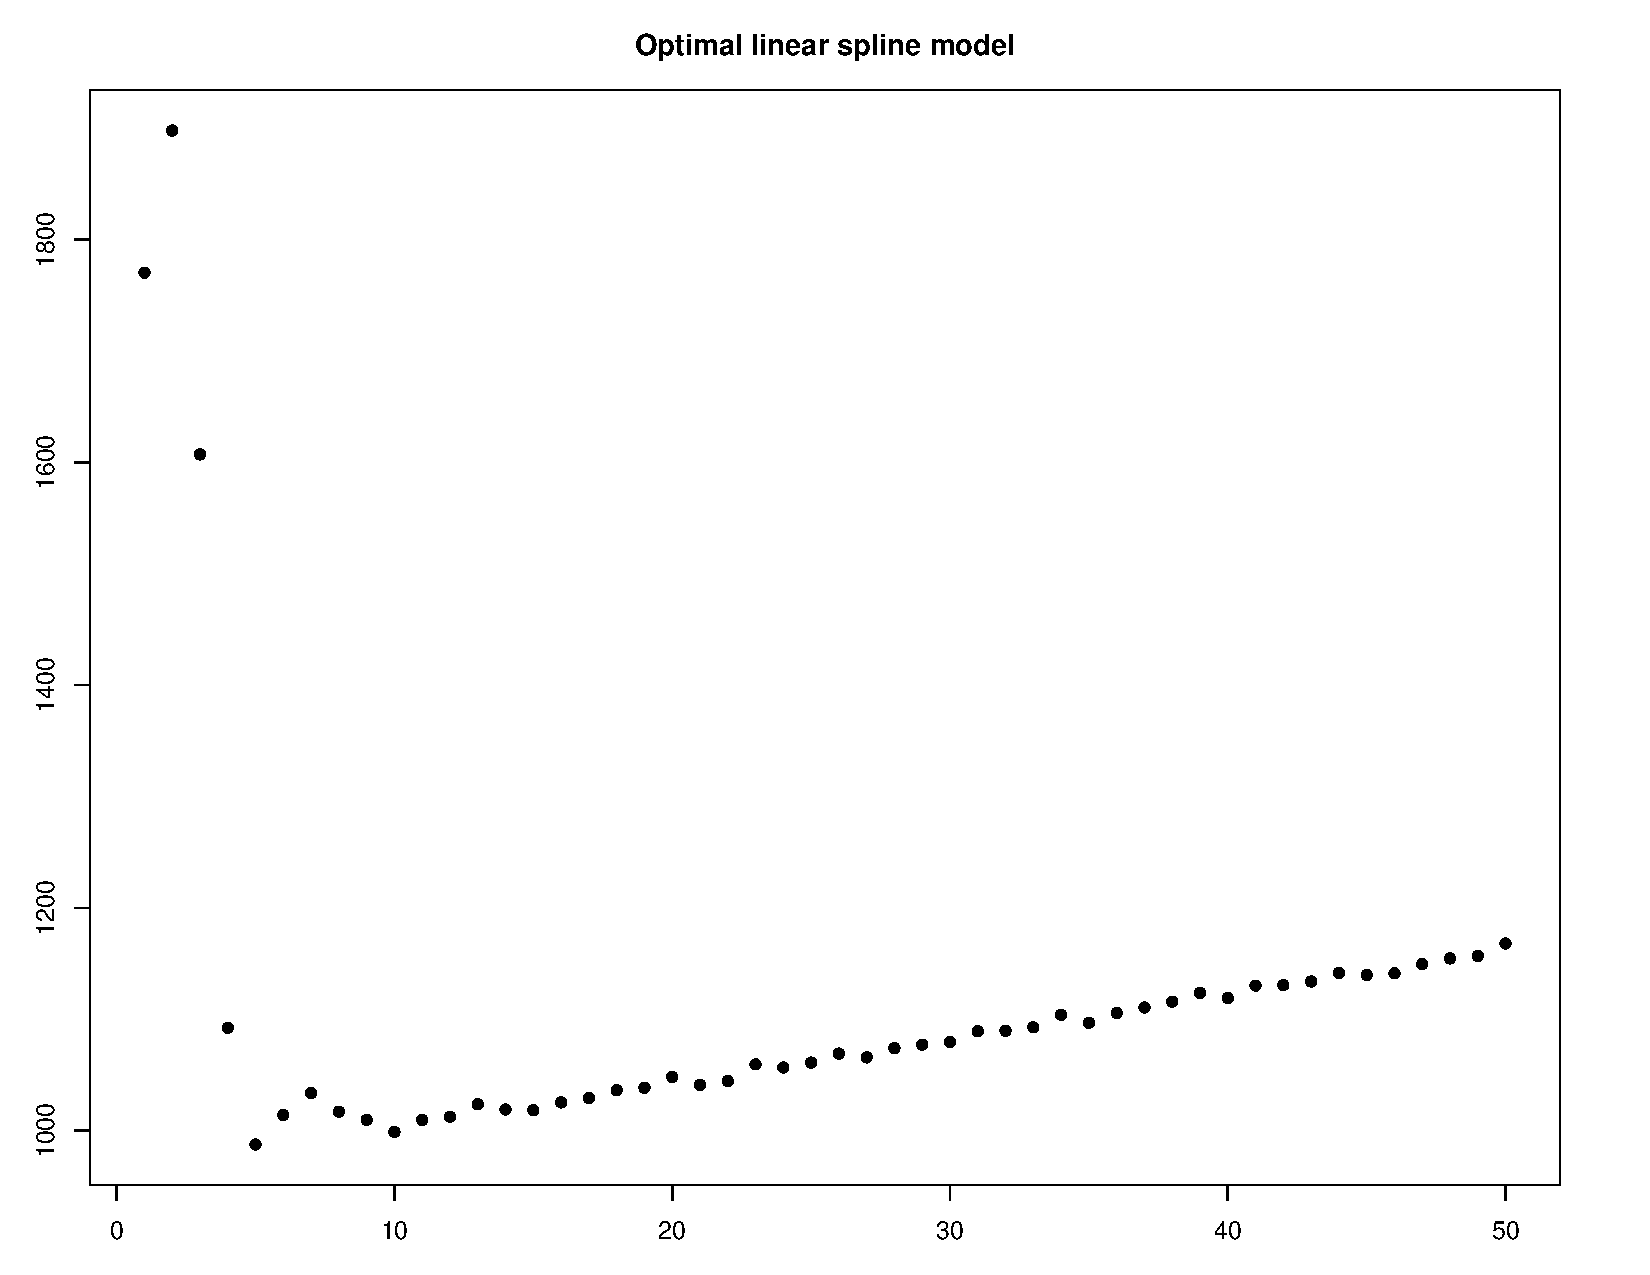
\includegraphics[scale=0.50]{figure2}
\end{center}
\end{figure}


\section{Kernel regression}
In this section, we are going to determine the optimal bandwidth for Kernel regression models. The idea is essentially the same as Section 3. 
\begin{Schunk}
\begin{Sinput}
> sortdat = dat[order(xx),]
> B = 200
> k2 = 20
> err = rep(0, times = k2)
> Errhat = rep(0, times = k2)
> h = seq(from = 0.1, to = 2, length.out = k2)
> for (k in 1:k2){
+   knmodel = ksmooth(sortdat$xx, sortdat$yy, 'normal', bandwidth = h[k], x.points=sortdat$xx)
+   yhat = knmodel$y
+   err[k] = sum((yhat-yy)^2)
+   boot = matrix(0, nrow = n, ncol = B)
+   for (j in 1:B){
+     boot[,j] = yhat + rnorm(n, 0, sigmahat)
+   }
+   boot_star = rep(0, times = n)
+   for (i in 1:n){
+     boot_star[i] = mean(boot[i,])
+   }
+   covhat = rep(0, times=B)
+   for (j in 1:B){
+     newdat = data.frame(x=sortdat$xx, y=boot[,j])
+     knmodelnew = ksmooth(newdat$x, newdat$y, 'normal', bandwidth = h[k], x.points=newdat$x)
+     muhatstar = knmodelnew$y
+     covhat[j] = sum(muhatstar*(boot[,j]-boot_star))/(B-1)
+   }
+   Errhat[k] = err[k]+2*sum(covhat)
+ }
> pdf("figure3.pdf",width=11,height=8.5) ;
> par(mar = c(3, 3, 3, 3)) 
> plot(h, Errhat, main="Optimal kernel regression model",pch=16,
+      xlab = "Bandwidth", ylab = "Estimated error")
\end{Sinput}
\end{Schunk}
We get the optimal bandwidth is $2$. One thing to notice is that the fitting result of kernel regression is very bad here and the estimated error keeps decreasing as the bandwidth increasing. Fitting this set of data using kernel regression is questionable and the optimal kernel regressio model derived in this setting is not trustworthy. 
\begin{figure}
\begin{center}
\caption{Estimated errors of the linear spline models with different number of knots}
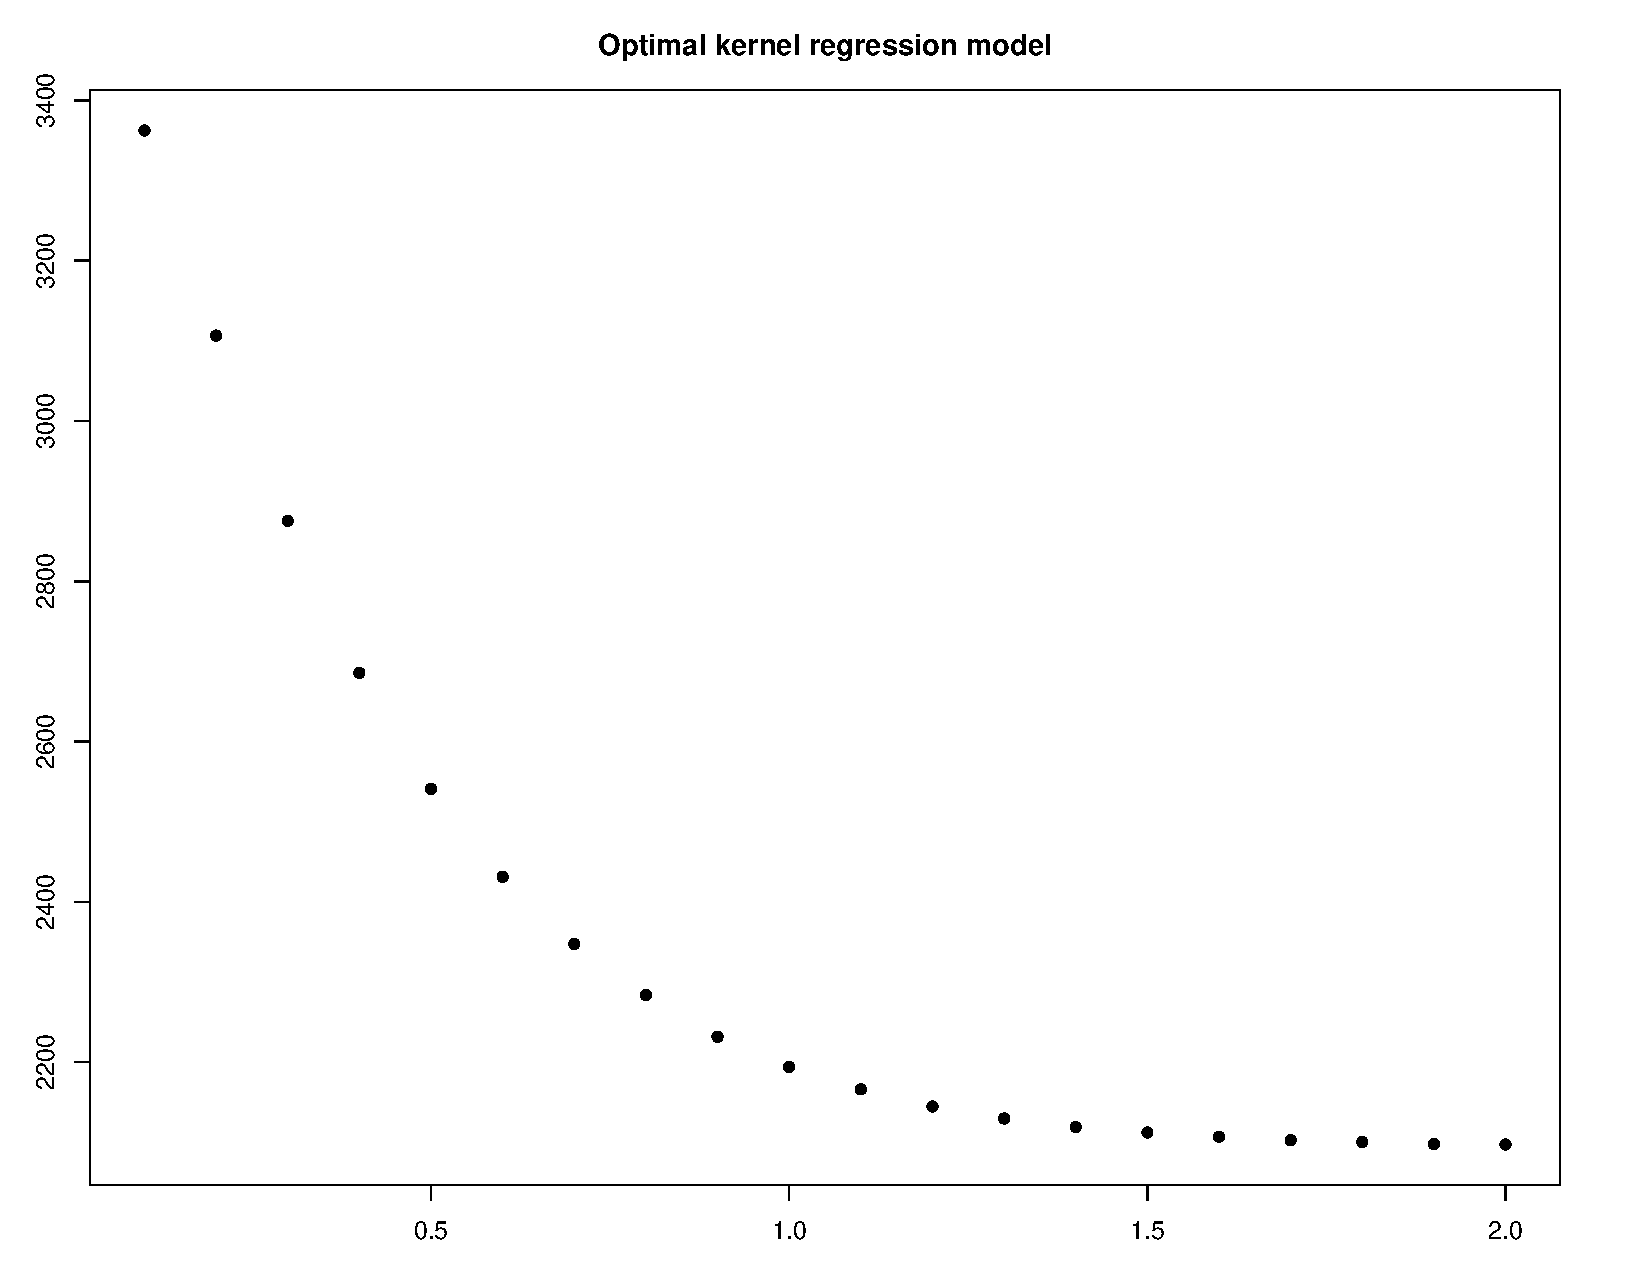
\includegraphics[scale=0.50]{figure3}
\end{center}
\end{figure}

\section{Lowess}
In this section, we are going to find the optimal locally weighted regression (Lowess) by Efron's procedure.
\begin{Schunk}
\begin{Sinput}
> B = 200
> k2 = 20
> err = rep(0, times = k2)
> Errhat = rep(0, times = k2)
> h = seq(from = 0.1, to = 1, length.out = k2)
> for (k in 1:k2){
+   lowessmd = loess(yy~xx, dat, span = h[k])
+   yhat = lowessmd$y
+   err[k] = sum(residuals(lowessmd)^2)
+   boot = matrix(0, nrow = n, ncol = B)
+   for (j in 1:B){
+     boot[,j] = yhat + rnorm(n, 0, sigmahat)
+   }
+   boot_star = rep(0, times = n)
+   for (i in 1:n){
+     boot_star[i] = mean(boot[i,])
+   }
+   covhat = rep(0, times=B)
+   for (j in 1:B){
+     newdat = data.frame(x=dat$xx, y=boot[,j])
+     lowessmdnew = loess(y~x, newdat, span = h[k])
+     muhatstar = lowessmdnew$y
+     covhat[j] = sum(muhatstar*(boot[,j]-boot_star))/(B-1)
+   }
+   Errhat[k] = err[k]+2*sum(covhat)
+ }
> pdf("figure4.pdf",width=11,height=8.5) ;
> par(mar = c(3, 3, 3, 3)) 
> plot(h, Errhat, main="Optimal Lowess model",pch=16,
+      xlab = "Span", ylab = "Estimated error")
\end{Sinput}
\end{Schunk}
We get the optimal bandwidth is $0.05$.
\begin{figure}
\begin{center}
\caption{Estimated errors of Lowess models with different spans}
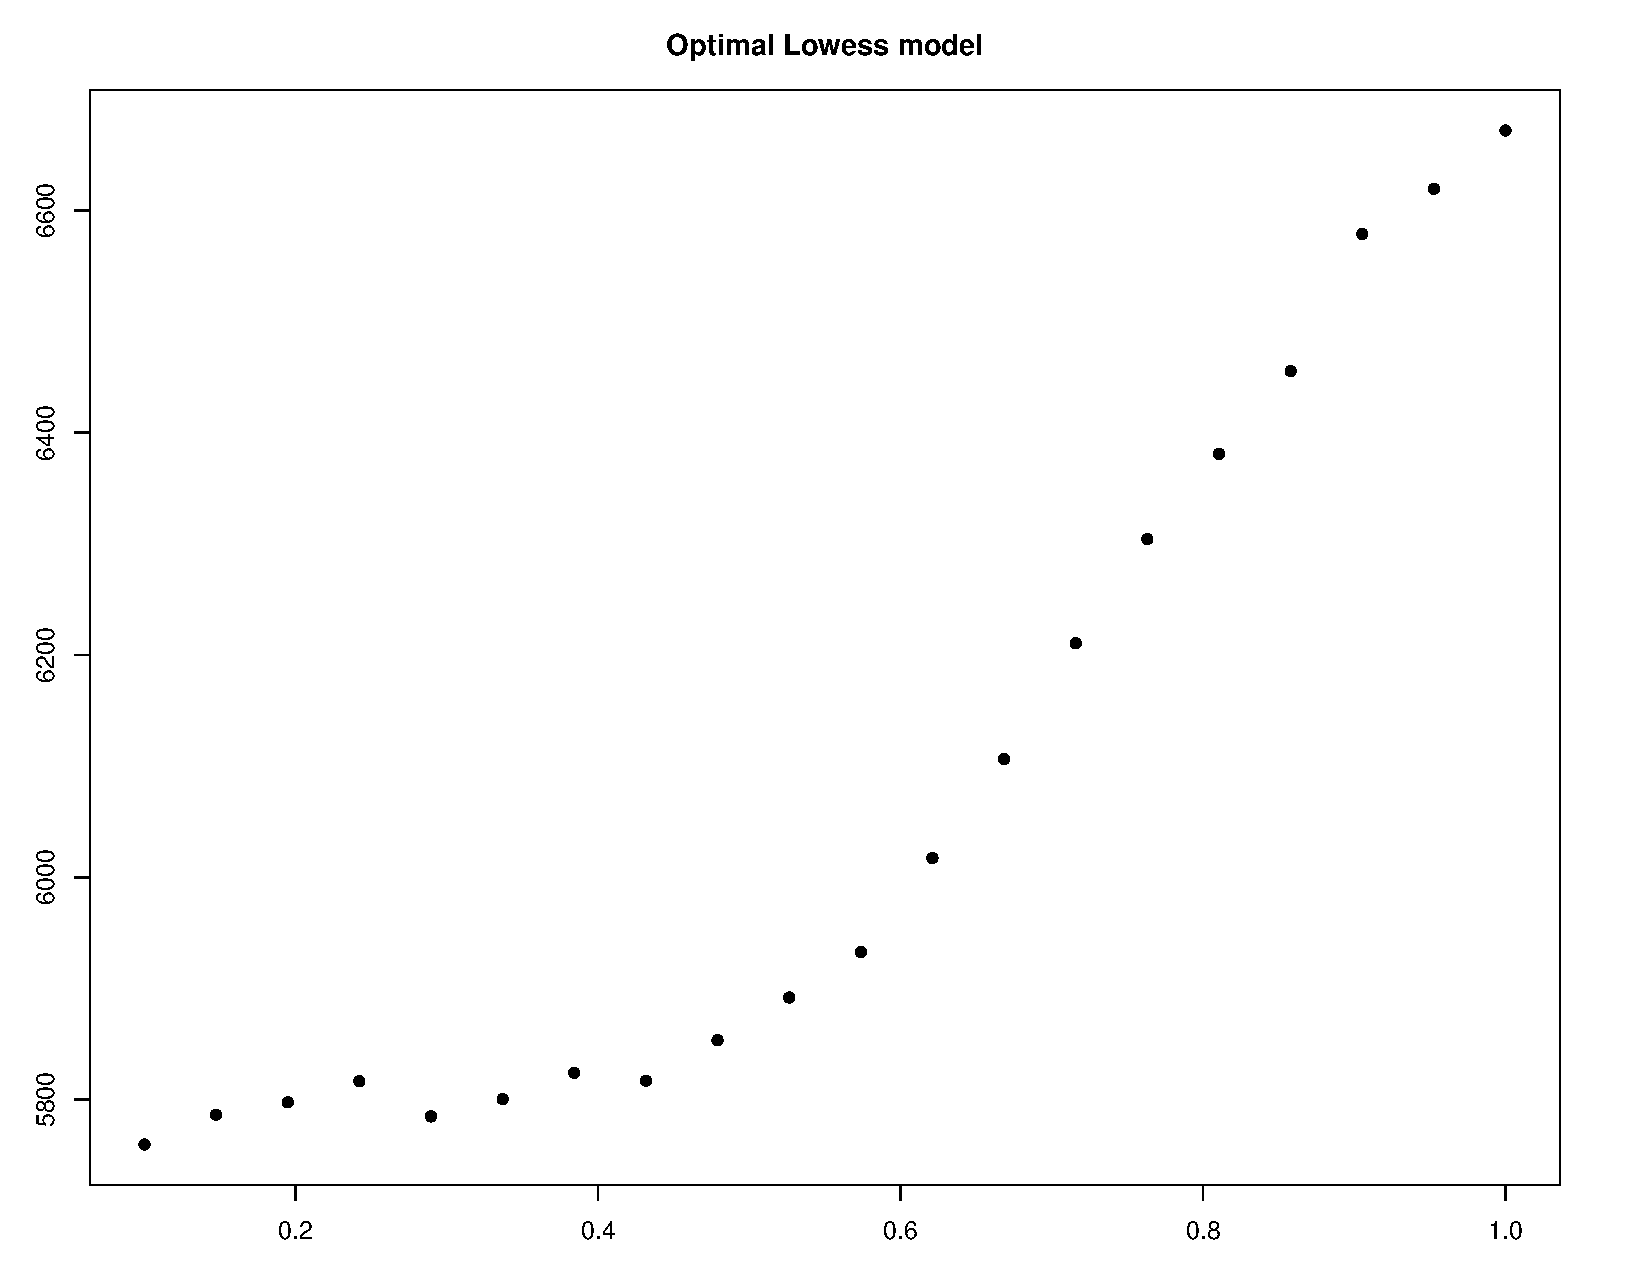
\includegraphics[scale=0.50]{figure4}
\end{center}
\end{figure}

\end{document}
